\chapter{سرعات التفاعلات}\label{ch:g12:reaction-rates}

قارورة حليب متروكة على طاولة المطبخ تحمض في يومين أو
ثلاثة؛ وفي الثلاجة تبقى صالحة أكثر من أسبوع. وتحترق مفرقعة نارية في
جزء من الثانية، بينما يتآكل تمثال من الحجر الجيري في حديقة عامة
على مدى قرون. فالمعادلات الموزونة وجداول التقدم تقول ما يعطيه
التفاعل وكم يعطي؛ ولا تقول شيئًا عن سرعته. وهذا الفصل
يقيس سرعة التفاعلات، ويكتشف ما يتحكم فيها،
ويصف أبسط طريقة يتباطأ بها التفاعل وهو يجري.

\begin{recall}
تركيز \omterm{def:g2:mixing-and-dissolving:dissolve}{المحلول} (\cref{ch:g10:concentration-and-dilution})
\omterm{def:g10:reaction-progress-table:extent}{وتقدم التفاعل} (\cref{ch:g10:reaction-progress-table}).
\omterm{def:g11:absorbance:absorbance}{وامتصاصية} \omterm{def:g2:mixing-and-dissolving:dissolve}{المحلول} المخفف متناسبة مع تركيز
النوع الملوّن (\cref{ch:g11:absorbance}). \omterm{def:g11:titration:titration}{والمعايرة} تقيس
كمية \omterm{def:g6:pure-substances-and-mixtures:species}{نوع كيميائي} (\cref{ch:g11:titration}).
\end{recall}

\begin{omfigure}
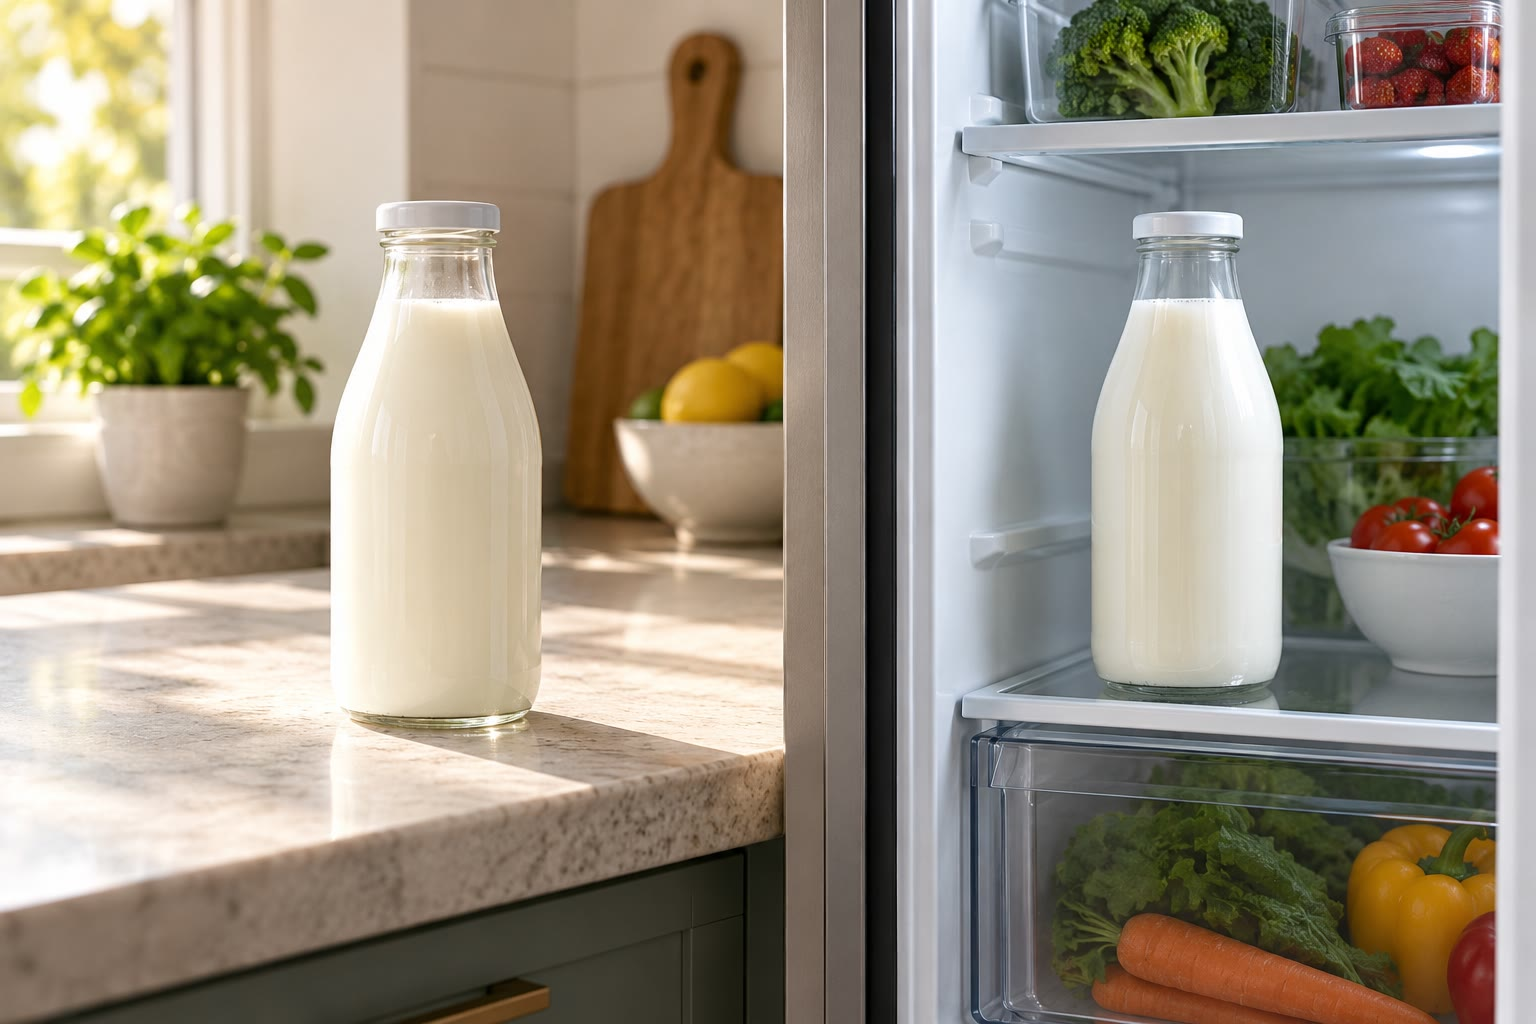
\includegraphics[width=0.48\linewidth]{images/book1/ai/g12-milk-counter-fridge.jpg}

{\small الحليب نفسه، على الطاولة وفي الثلاجة: التفاعلات
التي تحمّضه أبطأ في البرد.}
\end{omfigure}

\section{متابعة التفاعل في الزمن}

بعض التفاعلات ينتهي حالما تلتقي \omterm{def:g7:chemical-reactions:reactant}{المتفاعلات}: ترسيب
كلوريد الفضة، وتفاعل حمض مع قاعدة. وبعضها الآخر يستغرق
دقائق أو ساعات أو سنوات. ولدراسة تفاعل بطيء، يقيس الكيميائيون
تركيز \omterm{def:g7:chemical-reactions:reactant}{متفاعل} أو \omterm{def:g7:chemical-reactions:reactant}{ناتج} في أوقات منتظمة. فيمكنهم أن
\begin{itemize}
  \item يأخذوا عيّنات صغيرة، ويوقفوا التفاعل في كل منها، ويعايروها؛
  \item يقيسوا \omterm{def:g11:absorbance:absorbance}{امتصاصية} \omterm{def:g2:mixing-and-dissolving:dissolve}{المحلول}، حين يكون أحد \omterm{def:g7:chemical-reactions:reactant}{المتفاعلات} أو أحد
        \omterm{def:g7:chemical-reactions:reactant}{النواتج} ملوّنًا؛
  \item يقيسوا ضغط الغاز المنطلق أو حجمه، أو
        موصلية \omterm{def:g2:mixing-and-dissolving:dissolve}{محلول} تتغير أيوناته.
\end{itemize}

\begin{definition}[الإيقاف بالتبريد]\label{def:g12:reaction-rates:quenching}
\emph{الإيقاف بالتبريد}\index{إيقاف بالتبريد} لعيّنة هو إيقاف التفاعل فيها، أو
إبطاؤه إبطاءً شديدًا جدًا، لحظة أخذها، عادةً بتبريدها
فجأةً وتخفيفها، بحيث يمكن قياس تركيبها
على مهل.
\end{definition}

\begin{inthelab}[إيقاف التفاعل في عيّنة]
كل خمس دقائق، يؤخذ \qty{10.0}{mL} من \omterm{def:g6:pure-substances-and-mixtures:mixture}{خليط} التفاعل بماصة
ويُصبّ في كأس فيها نحو \qty{40}{mL} من
الماء المثلج. فبعد أن يُخفَّف خمس مرات ويُبرَّد قرب
\qty{0}{\celsius}، يصير التفاعل بطيئًا إلى حد يمكن معه اعتباره
متوقفًا؛ ثم تُعايَر العيّنة. ووقت العيّنة هو الوقت الذي
صُبّت فيه في الماء المثلج، لا وقت \omterm{def:g11:titration:titration}{المعايرة}.
\end{inthelab}

\begin{omfigure}
\begin{tikzpicture}[font=\small, scale=0.8]
  \pic[transform shape] at (0,0) {erlenmeyer={0.4}{orange!25}};
  \node[anchor=north, align=center] at (0,-0.15) {خليط\\ التفاعل};
  \pic[transform shape, rotate=-35] at (1.4,1.2) {pipette={0.6}{orange!25}};
  \draw[omProp, very thick, -{Stealth}] (1.6,0.8) -- (2.9,0.8);
  \node[anchor=south] at (2.25,0.85) {\qty{10.0}{mL}};
  \pic[transform shape] at (4,0) {beaker={0.55}{cyan!12}};
  \foreach \p in {(3.6,0.4),(4.2,0.6),(3.9,0.85),(4.4,0.3)}
    \draw[black!30, fill=white] \p ++(-0.1,-0.08) rectangle ++(0.2,0.16);
  \node[anchor=north, align=center] at (4,-0.15) {ماء مثلج:\\ التفاعل متوقف};
  \draw[omProp, very thick, -{Stealth}] (5.1,0.8) -- (6.4,0.8);
  \pic[transform shape] at (7.5,0) {erlenmeyer={0.35}{orange!12}};
  \pic[transform shape] at (7.5,2.75) {burette={0.7}{violet!45}};
  \node[anchor=north, align=center] at (7.5,-0.15) {معايرة\\ العيّنة};
\end{tikzpicture}

{\small متابعة تفاعل بأخذ العيّنات: خذ عيّنة، وأوقف التفاعل فيها بالتبريد، ثم
قِسها على مهل.}
\end{omfigure}

\section{العوامل الحركية}

\begin{definition}[العامل الحركي]\label{def:g12:reaction-rates:kinetic-factor}
\emph{العامل الحركي}\index{عامل حركي} مقدار يغيّر
سرعة التفاعل دون أن يغيّر ما يعطيه التفاعل:
درجة الحرارة، وتراكيز \omterm{def:g7:chemical-reactions:reactant}{المتفاعلات}، ومساحة التماس
بين متفاعلات في أطوار مختلفة، ووجود حفّاز
(الفصل التالي).
\end{definition}

\begin{proposition}[أسخن، وأشد تركيزًا، وأدق: فأسرع]\label{prop:g12:reaction-rates:factors}
يكون التفاعل عمومًا أسرع حين تكون درجة الحرارة أعلى، وحين تكون
\omterm{def:g7:chemical-reactions:reactant}{المتفاعلات} أشد تركيزًا، وحين يكون \omterm{def:g7:chemical-reactions:reactant}{المتفاعل} الصلب
أدق تجزئة.
\end{proposition}

\begin{proof}
نقبله، مع صورة: يجب على الجسيمات المتفاعلة أن تلتقي، وأن تلتقي بقوة
كافية. فتركيزها يجعل اللقاءات أكثر تواترًا؛ وتجزئة الصلب
تتيح سطحًا أكبر للقاء؛ والتسخين يجعلها تتحرك أسرع، فتلتقي
أكثر، والأهم أن نسبة أكبر من اللقاءات تكون نشيطة بما يكفي
لكسر الروابط.
\end{proof}

\begin{example}[ثلاث حالات يومية]\label{ex:g12:reaction-rates:everyday}
يبقى الغذاء صالحًا مدة أطول في الثلاجة ومدة أطول بكثير في المجمّد: فالتفاعلات
التي تفسده تتباطأ في البرد. وغبار الدقيق الناعم في \omterm{def:g4:air-a-mixture-of-gases:air}{هواء}
مطحنة قد ينفجر، بينما لا يفعل كيس الدقيق إلا أن يحترق ببطء: التفاعل نفسه،
ومساحة تماس هائلة. والقرص الفوار في الماء \omterm{def:g2:mixing-and-dissolving:dissolve}{يذوب}
أسرع إذا سُحق أولًا.
\end{example}

\begin{omfigure}
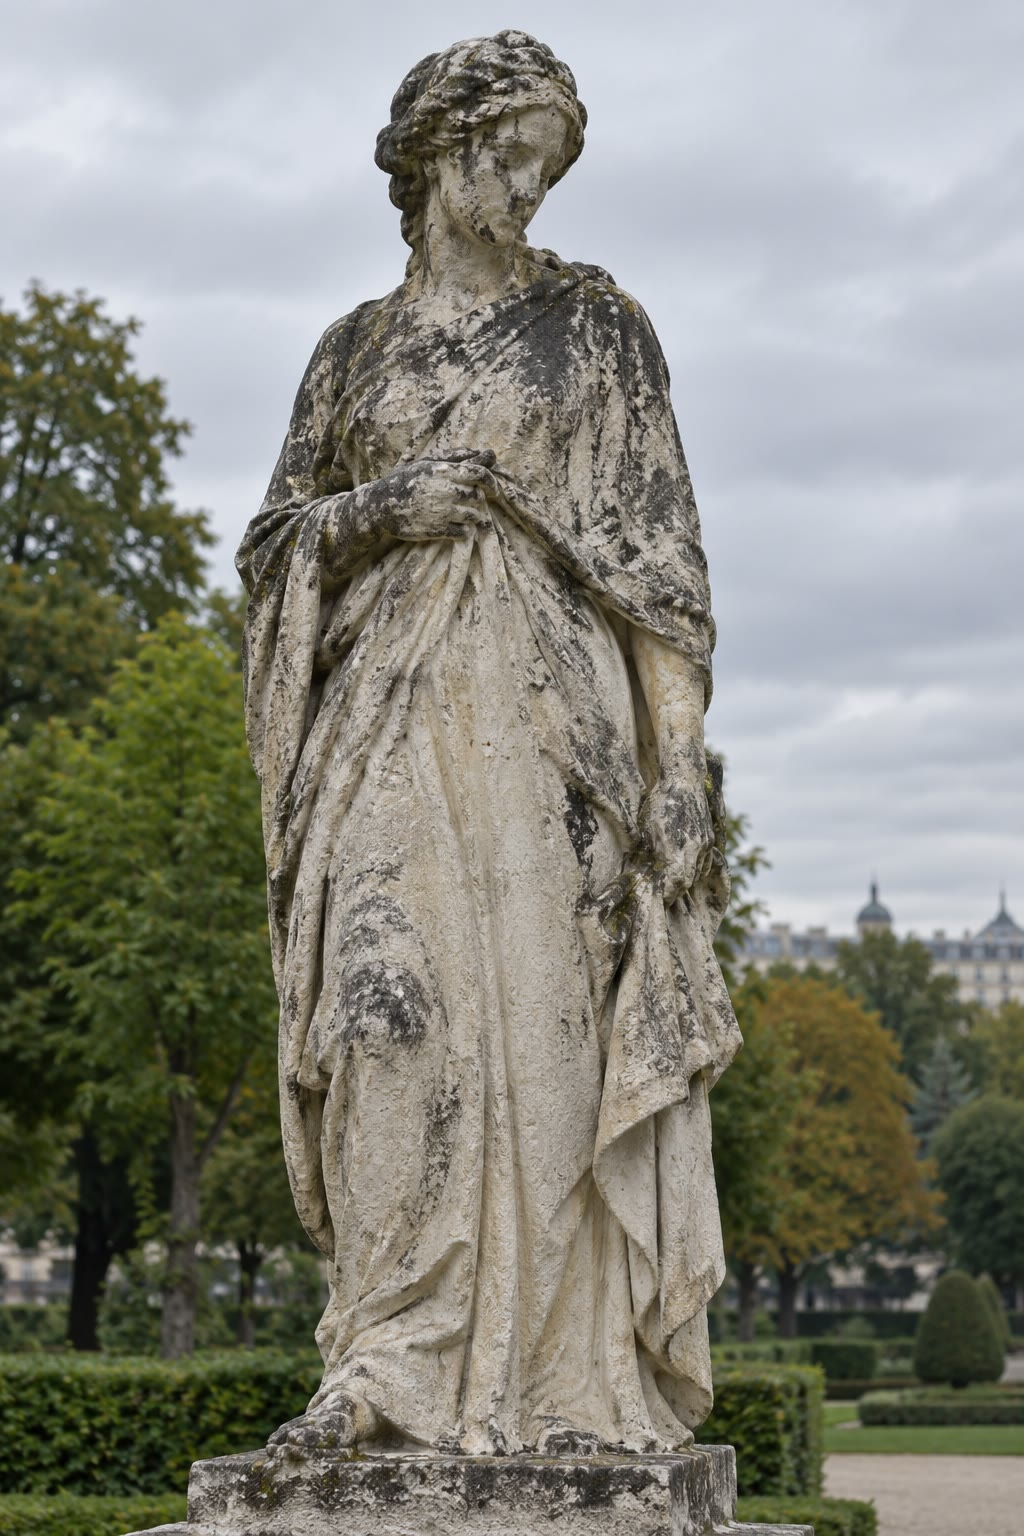
\includegraphics[width=0.42\linewidth,height=6cm,keepaspectratio]{images/book1/ai/g12-weathered-statue.jpg}

{\small تمثال من الحجر الجيري تآكل بفعل المطر: تفاعل يستغرق
قرونًا.}
\end{omfigure}

\section{سرعتا الاختفاء والظهور}

\begin{definition}[سرعة الاختفاء، سرعة الظهور]\label{def:g12:reaction-rates:rate}
في \omterm{def:g2:mixing-and-dissolving:dissolve}{محلول} حجمه ثابت، \emph{سرعة اختفاء}\index{سرعة الاختفاء}
\omterm{def:g7:chemical-reactions:reactant}{متفاعل} A عند اللحظة $t$ هي
\[
  v_A(t) = -\frac{d[\ce{A}]}{dt},
\]
و\emph{سرعة ظهور}\index{سرعة الظهور} \omterm{def:g7:chemical-reactions:reactant}{ناتج}
P هي $v_P(t) = \dfrac{d[\ce{P}]}{dt}$. وكلتاهما موجبة، بالوحدة
\si{mol.L^{-1}.min^{-1}} (أو لكل ثانية).
\end{definition}


\begin{method}[قراءة سرعة من مماس]\label{met:g12:reaction-rates:tangent}
\begin{enumerate}
  \item على منحنى $[\ce{A}]$ بدلالة $t$، ارسم المماس عند
        اللحظة المختارة.
  \item اقرأ نقطتين متباعدتين على المماس واحسب ميله،
        $\Delta[\ce{A}] / \Delta t$.
  \item \omterm{def:g12:reaction-rates:rate}{سرعة الاختفاء} هي معاكس هذا الميل (وللناتج،
        الميل نفسه).
\end{enumerate}
\end{method}

\begin{omfigure}
\begin{tikzpicture}
\begin{axis}[width=0.8\linewidth, height=6.4cm, xmin=0, xmax=60, ymin=0,
    ymax=11, xlabel={\babelsublr{$t$ (\si{min})}}, ylabel={\babelsublr{$[\ce{A}]$ (\si{mmol/L})}},
    axis lines*=left, ymajorgrids, xmajorgrids, grid style={gray!20},
    tick label style={font=\small}, label style={font=\small},
    legend style={font=\small, at={(0.98,0.97)}, anchor=north east,
    draw=none, fill=white}, legend cell align=left]
  \addplot[very thick, omDef] table[x=t, y=A1] {figdata/out/grade-12-reaction-rates-a.dat};
  \addplot[very thick, omThm] table[x=t, y=A2] {figdata/out/grade-12-reaction-rates-a.dat};
  \addplot[thick, dashed, omProp, restrict y to domain=0:11] table[x=t, y=tangent]
    {figdata/out/grade-12-reaction-rates-a.dat};
  \legend{{$k = \qty{0.050}{min^{-1}}$}, {\foreignlanguage{arabic}{$k = \qty{0.100}{min^{-1}}$، أسخن}},
    {\foreignlanguage{arabic}{المماس عند $t = 0$}}}
  \addplot[densely dotted, black!60] coordinates {(0,5) (13.86,5) (13.86,0)};
  \addplot[densely dotted, black!60] coordinates {(6.93,5) (6.93,0)};
  \node[font=\small, anchor=south west] at (axis cs:14.6,5.4) {$t_{1/2} = \qty{13.9}{min}$};
  \node[font=\small, anchor=south east] at (axis cs:6.7,0.2) {\qty{6.9}{min}};
\end{axis}
\end{tikzpicture}

{\small تركيز \omterm{def:g7:chemical-reactions:reactant}{متفاعل} A بدلالة الزمن، للتفاعل نفسه
من الرتبة الأولى عند درجتي حرارة. والمماس عند $t = 0$ (المتقطع)
يعطي السرعة الابتدائية؛ والخطوط المنقّطة تحدد أزمنة نصف التفاعل.}
\end{omfigure}

\begin{example}[السرعة الابتدائية]\label{ex:g12:reaction-rates:initial}
على المنحنى الأزرق، يمتد المماس عند $t = 0$ من \qty{10.0}{mmol/L} عند
$t = 0$ إلى $0$ عند $t = \qty{20}{min}$: فميله
$-10.0/20 = \qty{-0.50}{mmol.L^{-1}.min^{-1}}$، إذن \omterm{def:g12:reaction-rates:rate}{سرعة الاختفاء}
الابتدائية \qty{0.50}{mmol.L^{-1}.min^{-1}}. ثم يتسطح المنحنى
وتنخفض السرعة: فالتفاعل يتباطأ كلما استُهلك A.
\end{example}

\section{التفاعلات من الرتبة الأولى}

\begin{definition}[التفاعل من الرتبة الأولى، ثابت السرعة]\label{def:g12:reaction-rates:first-order}
يكون التفاعل \emph{تفاعلًا من الرتبة الأولى}\index{تفاعل من الرتبة الأولى}
بالنسبة إلى A إذا كانت سرعة اختفائه متناسبة مع
تركيز A في كل لحظة:
\[
  -\frac{d[\ce{A}]}{dt} = k\,[\ce{A}] .
\]
والثابت الموجب $k$، بالوحدة \si{min^{-1}} أو \si{s^{-1}}، هو
\emph{ثابت السرعة}\index{ثابت السرعة}؛ ويتوقف على درجة الحرارة.
\end{definition}

\begin{proposition}[التناقص الأسي]\label{prop:g12:reaction-rates:exponential}
\omterm{def:g12:reaction-rates:first-order}{لتفاعل من الرتبة الأولى} تركيزه الابتدائي $[\ce{A}]_0$،
\[
  [\ce{A}](t) = [\ce{A}]_0\, e^{-kt} .
\]
\end{proposition}

\begin{proof}
للدالة $f(t) = [\ce{A}]_0 e^{-kt}$ المشتقة
$f'(t) = -k [\ce{A}]_0 e^{-kt} = -k f(t)$، فهي تحقق معادلة
السرعة، و$f(0) = [\ce{A}]_0$. أما أنها الدالة الوحيدة التي تحقق ذلك فنقبله
هنا (وهو يُبرهن في الرياضيات، للمعادلات $y' = ay$).
\end{proof}

\begin{method}[اختبار الرتبة الأولى]\label{met:g12:reaction-rates:test}
\begin{enumerate}
  \item انطلاقًا من القياسات، احسب $\ln [\ce{A}]$ (أو $\ln A$ في حالة
        \omterm{def:g11:absorbance:absorbance}{امتصاصية} متناسبة مع $[\ce{A}]$) عند كل لحظة.
  \item ارسم $\ln[\ce{A}]$ بدلالة $t$: فبما أن
        $\ln[\ce{A}] = \ln[\ce{A}]_0 - kt$، تقع النقاط على خط
        مستقيم إذا كان \omterm{def:g12:reaction-rates:first-order}{التفاعل من الرتبة الأولى}، وفقط إذا كان كذلك.
  \item ميل المستقيم يساوي $-k$.
\end{enumerate}
\end{method}

\section{زمن نصف التفاعل}

\begin{definition}[زمن نصف التفاعل]\label{def:g12:reaction-rates:half-life}
\emph{زمن نصف التفاعل}\index{زمن نصف التفاعل} $t_{1/2}$ هو المدة
التي يستغرقها تركيز \omterm{def:g7:chemical-reactions:reactant}{المتفاعل} المحِدّ لينخفض إلى نصف
قيمته الابتدائية.
\end{definition}

\begin{proposition}[زمن نصف التفاعل من الرتبة الأولى]\label{prop:g12:reaction-rates:half-life}
\omterm{def:g12:reaction-rates:first-order}{لتفاعل من الرتبة الأولى}،
\[
  t_{1/2} = \frac{\ln 2}{k},
\]
مهما كان التركيز الابتدائي؛ وبعد $n$ من أزمنة نصف التفاعل، يكون
التركيز قد قُسم على $2^n$.
\end{proposition}

\begin{proof}
العلاقة $[\ce{A}]_0 e^{-k t_{1/2}} = [\ce{A}]_0 / 2$ تعطي $e^{-k t_{1/2}} = 1/2$،
إذن $k t_{1/2} = \ln 2$. وكل زمن نصف تفاعل إضافي يضرب
التركيز في $e^{-k t_{1/2}} = 1/2$ من جديد.
\end{proof}


\begin{example}[قراءة أزمنة نصف التفاعل]\label{ex:g12:reaction-rates:half-lives}
لقيمة $k = \qty{0.050}{min^{-1}}$، $t_{1/2} = 0.693 / 0.050 =
\qty{13.9}{min}$: فينخفض التركيز من 10.0 إلى 5.0، ثم 2.5،
ثم \qty{1.25}{mmol/L} عند 13.9 و27.7 و\qty{41.6}{min}. والتجربة الأسخن،
وفيها $k$ أكبر بمرتين، لها نصف \omterm{def:g12:reaction-rates:half-life}{زمن نصف التفاعل}، \qty{6.9}{min}، كما
يبيّن الشكل.
\end{example}

\begin{remark}[أزمنة نصف في مواضع أخرى]\label{rem:g12:reaction-rates:radioactive}
تُستعمل الكلمة نفسها في الفيزياء للنوى المشعة، التي يتناقص عددها
بالطريقة الأسية نفسها: فالتفكك الإشعاعي يسلك سلوك
\omterm{def:g12:reaction-rates:first-order}{تفاعل من الرتبة الأولى}. ويعالجه كتاب الفيزياء.
\end{remark}

\begin{omfigure}
\begin{minipage}{0.49\linewidth}
\begin{tikzpicture}
\begin{axis}[width=\linewidth, height=5.4cm, xmin=0, xmax=26, ymin=0,
    ymax=0.85, xlabel={\babelsublr{$t$ (\si{min})}}, ylabel={\foreignlanguage{arabic}{الامتصاصية $A$}},
    axis lines*=left, ymajorgrids, grid style={gray!20},
    tick label style={font=\scriptsize}, label style={font=\small}]
  \addplot[only marks, mark=*, mark size=1.8pt, omDef] table[x=t, y=A]
    {figdata/out/grade-12-reaction-rates-b.dat};
  \addplot[thick, omProp, domain=0:26, samples=60] {0.8*exp(-0.11552*x)};
\end{axis}
\end{tikzpicture}
\end{minipage}\hfill
\begin{minipage}{0.49\linewidth}
\begin{tikzpicture}
\begin{axis}[width=\linewidth, height=5.4cm, xmin=0, xmax=26, ymin=-3.4,
    ymax=0, xlabel={\babelsublr{$t$ (\si{min})}}, ylabel={\babelsublr{$\ln A$}}, axis lines*=left,
    ymajorgrids, grid style={gray!20}, tick label style={font=\scriptsize},
    label style={font=\small}]
  \addplot[only marks, mark=*, mark size=1.8pt, omDef] table[x=t, y=lnA]
    {figdata/out/grade-12-reaction-rates-b.dat};
  \addplot[thick, omProp, domain=0:26] {-0.2231-0.11552*x};
\end{axis}
\end{tikzpicture}
\end{minipage}

{\small بهتان البنفسج البلوري في \omterm{def:g9:acids-bases-ph:acidic}{محلول قاعدي} (معطيات مسألة نهاية
الأسبوع). يسارًا: تنخفض \omterm{def:g11:absorbance:absorbance}{الامتصاصية} وفق دالة أسية.
يمينًا: $\ln A$ بدلالة $t$ خط مستقيم ميله
$-\qty{0.116}{min^{-1}}$: \omterm{def:g12:reaction-rates:first-order}{فالتفاعل من الرتبة الأولى} بالنسبة إلى الصبغة.}
\end{omfigure}

\section{تمارين}

\begin{exercise}[$\star$]\label{exo:g12:reaction-rates:1}
سمِّ \omterm{def:g12:reaction-rates:kinetic-factor}{العامل الحركي} الفاعل في كل حالة: الثلاجة تحفظ الغذاء؛
السكر المسحوق \omterm{def:g2:mixing-and-dissolving:dissolve}{يذوب} أسرع من القطعة؛ الحمض الأشد تركيزًا يهاجم
الخارصين أسرع؛ التفاحة المقطوعة تسمرّ أسرع في الصيف.
\end{exercise}

\begin{exercise}[$\star$]\label{exo:g12:reaction-rates:2}
اقرأ على شكل $[\ce{A}]$ بدلالة الزمن \omterm{def:g12:reaction-rates:half-life}{زمن نصف التفاعل} لكل تجربة.
وما قيمة $[\ce{A}]$ على المنحنى الأزرق بعد زمني نصف تفاعل؟
\end{exercise}

\begin{exercise}[$\star$]\label{exo:g12:reaction-rates:3}
يمر مماس لمنحنى \omterm{def:g7:chemical-reactions:reactant}{ناتج} مرسوم عند $t = \qty{5}{min}$
بالنقطتين $(0, \qty{1.0}{mmol/L})$ و$(\qty{10}{min}, \qty{5.0}{mmol/L})$.
ما \omterm{def:g12:reaction-rates:rate}{سرعة ظهور} \omterm{def:g7:chemical-reactions:reactant}{الناتج} عند \qty{5}{min}؟
\end{exercise}

\begin{exercise}[$\star$]\label{exo:g12:reaction-rates:4}
لماذا تُصبّ العيّنة في ماء مثلج قبل معايرتها؟ ولماذا
يجب تسجيل وقت العيّنة عند صبّها، لا عند
معايرتها؟
\end{exercise}

\begin{exercise}[$\star$]\label{exo:g12:reaction-rates:5}
زمن نصف \omterm{def:g12:reaction-rates:first-order}{تفاعل من الرتبة الأولى} \qty{10}{min}. ما الكسر الذي
يبقى من \omterm{def:g7:chemical-reactions:reactant}{المتفاعل} بعد \qty{30}{min}؟ وبعد \qty{1}{h}؟
\end{exercise}

\begin{exercise}[$\star\star$]\label{exo:g12:reaction-rates:6}
تراكيز \omterm{def:g7:chemical-reactions:reactant}{متفاعل}، بالوحدة \si{mmol/L}: 8.00 عند \qty{0}{min}، و5.66
عند \qty{5}{min}، و4.00 عند \qty{10}{min}، و2.83 عند \qty{15}{min}، و2.00 عند
\qty{20}{min}. احسب $\ln[\ce{A}]$ عند كل لحظة وبيّن أن
\omterm{def:g12:reaction-rates:first-order}{التفاعل من الرتبة الأولى}. وجد $k$ \omterm{def:g12:reaction-rates:half-life}{وزمن نصف التفاعل}.
\end{exercise}

\begin{exercise}[$\star\star$]\label{exo:g12:reaction-rates:7}
\omterm{def:g12:reaction-rates:first-order}{لتفاعل من الرتبة الأولى} $t_{1/2} = \qty{25}{s}$. احسب $k$.
\end{exercise}

\begin{exercise}[$\star\star$]\label{exo:g12:reaction-rates:8}
لقيمتي $[\ce{A}]_0 = \qty{0.100}{mol/L}$ و$k = \qty{0.020}{min^{-1}}$،
احسب $[\ce{A}]$ بعد 10 و30 و\qty{100}{min}.
\end{exercise}

\begin{exercise}[$\star\star$]\label{exo:g12:reaction-rates:9}
على شكل $[\ce{A}]$ بدلالة الزمن، قدّر ميل المنحنى
الأزرق عند $t = \qty{13.9}{min}$ (ارسم مماسًا)، وقارنه
بالمقدار $-k[\ce{A}]$ عند تلك اللحظة.
\end{exercise}

\begin{exercise}[$\star\star$]\label{exo:g12:reaction-rates:10}
يتكوّن ثنائي اليود \ce{I2}، البني، ببطء في \omterm{def:g2:mixing-and-dissolving:dissolve}{محلول} عديم اللون. وترتفع
\omterm{def:g11:absorbance:absorbance}{الامتصاصية} من 0 نحو 0.60. اشرح لماذا يمكن استعمال \omterm{def:g11:absorbance:absorbance}{الامتصاصية}
لمتابعة $[\ce{I2}]$، وكيف تُقرأ \omterm{def:g12:reaction-rates:rate}{سرعة الظهور} عند لحظة
معيّنة على منحنى $A$ بدلالة $t$.
\end{exercise}

\begin{exercise}[$\star\star$]\label{exo:g12:reaction-rates:11}
تبدأ تجربتان للتفاعل نفسه من $[\ce{A}]_0 = 10$
و\qty{20}{mmol/L}. فإذا كان \omterm{def:g12:reaction-rates:first-order}{التفاعل من الرتبة الأولى}، فقارن سرعتيهما
الابتدائيتين وزمني نصف التفاعل فيهما.
\end{exercise}

\begin{exercise}[$\star\star\star$]\label{exo:g12:reaction-rates:12}
كم زمن نصف تفاعل يلزم \omterm{def:g12:reaction-rates:first-order}{لتفاعل من الرتبة الأولى} كي يصل
إلى \qty{1}{\percent} من متفاعله؟ وإلى \qty{0.1}{\percent}؟ أعطِ الصيغة
العامة للزمن اللازم للانخفاض إلى كسر $f$.
\end{exercise}

\begin{exercise}[$\star\star\star$]\label{exo:g12:reaction-rates:13}
لتفاعل $k = \qty{0.050}{min^{-1}}$ عند \qty{20}{\celsius}
و$k = \qty{0.100}{min^{-1}}$ عند \qty{30}{\celsius}. كم من الوقت يلزم
لاستهلاك \qty{90}{\percent} من \omterm{def:g7:chemical-reactions:reactant}{المتفاعل} عند كل درجة حرارة؟ وتقول
قاعدة تقريبية شائعة إن السرعة تتضاعف كل \qty{10}{\celsius}: فهل
يتبعها هذا التفاعل؟
\end{exercise}

\begin{exercise}[$\star\star\star$]\label{exo:g12:reaction-rates:14}
يُوقف التفاعل في عيّنة بصبّ \qty{5.0}{mL} منها في \qty{45}{mL} من الماء
المثلج. أعطِ سببين لصيرورة التفاعل أبطأ بكثير. وإذا كان
\omterm{def:g12:reaction-rates:first-order}{التفاعل من الرتبة الأولى} بالنسبة إلى كل من متفاعلين، فعلى أي عامل
يقسم \omterm{def:g10:concentration-and-dilution:dilution}{التخفيف} وحده السرعة؟
\end{exercise}

\begin{exercise}[$\star\star\star$]\label{exo:g12:reaction-rates:15}
بيّن، بالاشتقاق، أن \omterm{def:g12:reaction-rates:rate}{سرعة اختفاء} \omterm{def:g7:chemical-reactions:reactant}{المتفاعل} في \omterm{def:g12:reaction-rates:first-order}{تفاعل
من الرتبة الأولى} هي نفسها دالة أسية للزمن،
$v(t) = k[\ce{A}]_0 e^{-kt}$. ما السرعة الابتدائية؟ وبعد كم من الوقت تصير
السرعة نصف السرعة الابتدائية؟
\end{exercise}

\section{مسألة: الصبغة التي تبهت}

\begin{problem}[{مسألة نهاية الأسبوع --- البنفسج البلوري تزيل لونه أيونات
الهيدروكسيد: كم يلزم من الوقت حتى يكاد اللون يختفي؟}]
\label{pb:g12:reaction-rates:1}
تتفاعل الصبغة البنفسجية «البنفسج البلوري» مع \omterm{def:g9:ions:ion}{أيونات} الهيدروكسيد فتعطي
ناتجًا عديم اللون. وبوجود فائض كبير من الهيدروكسيد، لا تتوقف السرعة
إلا على تركيز الصبغة. وتُسجَّل \omterm{def:g11:absorbance:absorbance}{امتصاصية} \omterm{def:g2:mixing-and-dissolving:dissolve}{المحلول}
عند الطول الموجي الذي تمتص فيه الصبغة أكثر من غيره:
\begin{center}
\small
\begin{tabular}{l*{10}{c}}
\hline
$t$ (\si{min}) & 0 & 2 & 4 & 6 & 8 & 10 & 12 & 15 & 20 & 25 \\
$A$ & 0.800 & 0.639 & 0.501 & 0.402 & 0.315 & 0.255 & 0.199 & 0.143 &
0.078 & 0.046 \\
\hline
\end{tabular}
\end{center}

\medskip
\noindent\textbf{الجزء الأول --- \omterm{def:g11:absorbance:absorbance}{الامتصاصية} والتركيز.}
\begin{enumerate}
  \item لماذا تتناسب \omterm{def:g11:absorbance:absorbance}{الامتصاصية} مع تركيز
        الصبغة؟ وأي شرط يجب أن يحققه \omterm{def:g2:mixing-and-dissolving:dissolve}{المحلول}؟
  \item لماذا لا يُرى \omterm{def:g7:chemical-reactions:reactant}{الناتج}، العديم اللون، عند هذا الطول الموجي؟
  \item لماذا يُستعمل الهيدروكسيد بفائض كبير؟
  \item ماذا يُقرأ على المطياف الضوئي في نهاية
        التفاعل؟
\end{enumerate}

\medskip
\noindent\textbf{الجزء الثاني --- أهو من الرتبة الأولى؟}
\begin{enumerate}[resume]
  \item اقرأ \omterm{def:g12:reaction-rates:half-life}{زمن نصف التفاعل} مباشرة في الجدول.
  \item تحقق من أنه هو نفسه من $t = 6$ إلى $t = 12$ min.
  \item احسب $\ln A$ لكل لحظة.
  \item ارسم $\ln A$ بدلالة $t$ (أو استعمل شكل الفصل). ماذا
        تلاحظ؟ استنتج.
  \item احسب الميل من النقطتين عند 0 و\qty{20}{min}.
\end{enumerate}

\medskip
\noindent\textbf{الجزء الثالث --- \omterm{def:g12:reaction-rates:first-order}{ثابت السرعة}.}
\begin{enumerate}[resume]
  \item استنتج $k$.
  \item احسب \omterm{def:g12:reaction-rates:half-life}{زمن نصف التفاعل} من $k$، وقارن بالسؤال 5.
  \item احسب \omterm{def:g12:reaction-rates:rate}{سرعة الاختفاء} الابتدائية للصبغة، معبَّرًا عنها
        بسرعة تناقص \omterm{def:g11:absorbance:absorbance}{الامتصاصية}.
  \item كم يكون \omterm{def:g12:reaction-rates:half-life}{زمن نصف التفاعل} لو كانت \omterm{def:g11:absorbance:absorbance}{الامتصاصية} الابتدائية 0.400؟
\end{enumerate}

\medskip
\noindent\textbf{الجزء الرابع --- التنبؤ.}
\begin{enumerate}[resume]
  \item تنبأ \omterm{def:g11:absorbance:absorbance}{بالامتصاصية} عند \qty{30}{min}.
  \item في أي لحظة تنخفض \omterm{def:g11:absorbance:absorbance}{الامتصاصية} إلى 0.008، أي \qty{1}{\percent}
        من قيمتها الابتدائية؟
  \item كم زمن نصف تفاعل يمثل ذلك؟
  \item لا تعود العين ترى اللون تحت نحو $A = 0.010$. فمتى
        يبدو \omterm{def:g2:mixing-and-dissolving:dissolve}{المحلول} عديم اللون؟
  \item تُعاد التجربة عند درجة حرارة أعلى بمقدار \qty{10}{\celsius} فيصير
        \omterm{def:g12:reaction-rates:half-life}{زمن نصف التفاعل} \qty{3.0}{min}. فمتى تُبلغ نسبة \qty{1}{\percent}؟
  \item اذكر الجواب النهائي: كم زمن نصف تفاعل يلزم كي ينخفض اللون
        إلى \qty{1}{\percent} من قيمته الابتدائية، وكم دقيقة يمثل
        ذلك هنا؟
\end{enumerate}
\end{problem}
